\section{Containerization}

\begin{flushleft}

A Container is a software unit that packages an application along with all its dependencies including libraries, environment and tools necessary to run the application on any computing environment thereby allowing for easy migration from one computing environment to another. Docker provides an eco-system to create images, store them in a repository, run the application and monitor the application on a computing environment. Refer to documentation in \cite[3]
The layered architecture of a container-based system is as in [Fig.11] below based on the explanation from [3]
\end{flushleft}

\begin{figure}
    \centering
    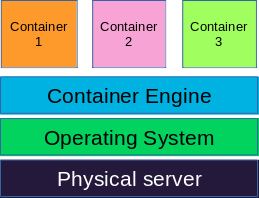
\includegraphics[width=0.5\textwidth]{container_layers}
    \label{fig:figure9}
    \caption{Components of Containerization}
\end{figure}

